%!TEX root = ../main.tex
\chapter{2.5维谐振腔的制备与测量} % (fold)
\label{cha:2_5维谐振腔的制备与测量}
	


        \section{器件测量与制备工艺概述} % (fold)
        \label{sec:制备工艺概述}

            由于2.5维谐振腔的电容部分由上下两层金属以及中间的介电层组成,工艺较为复杂,需要至少三步光刻来完成。而细小的电感部分则需要电子束曝光(EBL)来定义形状,再由蒸发镀膜完成。因此,总的制备工艺大致如下:

            \begin{enumerate}
                \item 通过光刻,磁控溅射蒸镀金属Nb,Lift off三步制作平面波导与三层电容的第一层
                \item 通过ALD生长Al$_2$O$_3$,或通过PECVD生长SiO$_2$或SiN$_x$作为三层电容的介电层
                \item 光刻定义掩膜后通过ICP刻蚀或湿法刻蚀介电层
                    \begin{enumerate}
                        \item 剩余的介电层仅遮盖住三层电容的底层
                    \end{enumerate}
                \item 利用光刻制作出三层电容的顶层图案并蒸镀金属,对准精度约1微米,Lift off
                \item 利用EBL制作微小电感图案
                    \begin{enumerate}
                        \item 电感图案将与三层电容的上下级板相连
                        \item 对准精度 100-1000 nm
                    \end{enumerate}
            \end{enumerate}


            每一步制备工艺的具体步骤与相关参数均在附录\ref{cha:fabrication}中给出。
            
        % subsection 制备工艺概述 (end)

        \section{光刻板的设计与改进} % (fold)
        \label{sec:光刻板的设计}

            由于制备工艺需要三步光刻,对于完整制备一个器件来说,需要的光刻板的图案为一组三个,分别对应\ref{sec:制备工艺概述}制备工艺概述中的前三步。第一步完成二维平面波导以及接地平面的制作,以及三维电容的第一层金属。第二步在生长介电材料后通过光刻制作掩膜覆盖住需要保留的电容的第二层介电层部分,并刻蚀掉没有被覆盖掉的电介质。第三部制作出电容最上层的金属。最后一步通过电子束曝光与蒸镀制作微小的电感部分,并各自与三维电容的上、下两层连接起来。光刻的三个步骤所需的模板作图如图所示
            

            \begin{figure}[h]
                \centering
                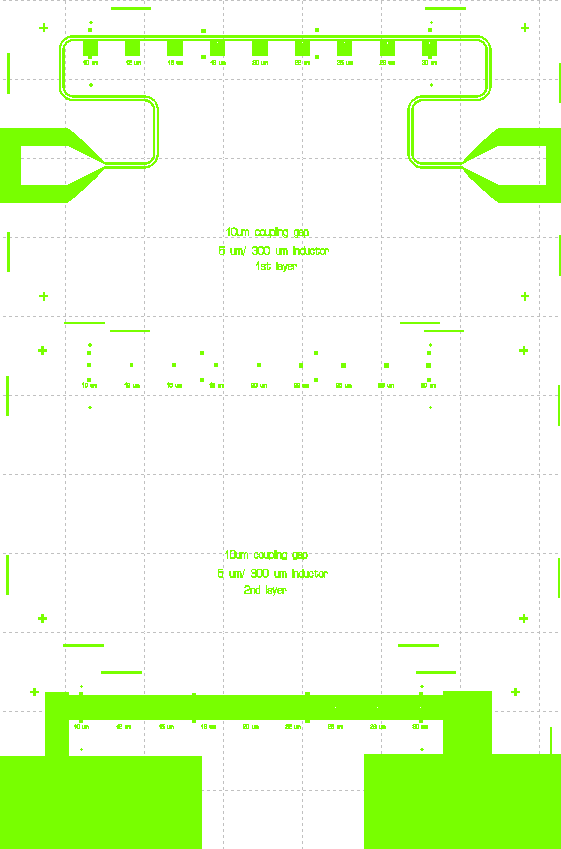
\includegraphics[width=3in]{one_group.png}
                \caption{制备一个器件所需的三个光刻步骤对应的一组三个模板图案}
                \label{fig:one_group}
            \end{figure}

            \begin{figure}[h]
                \centering
                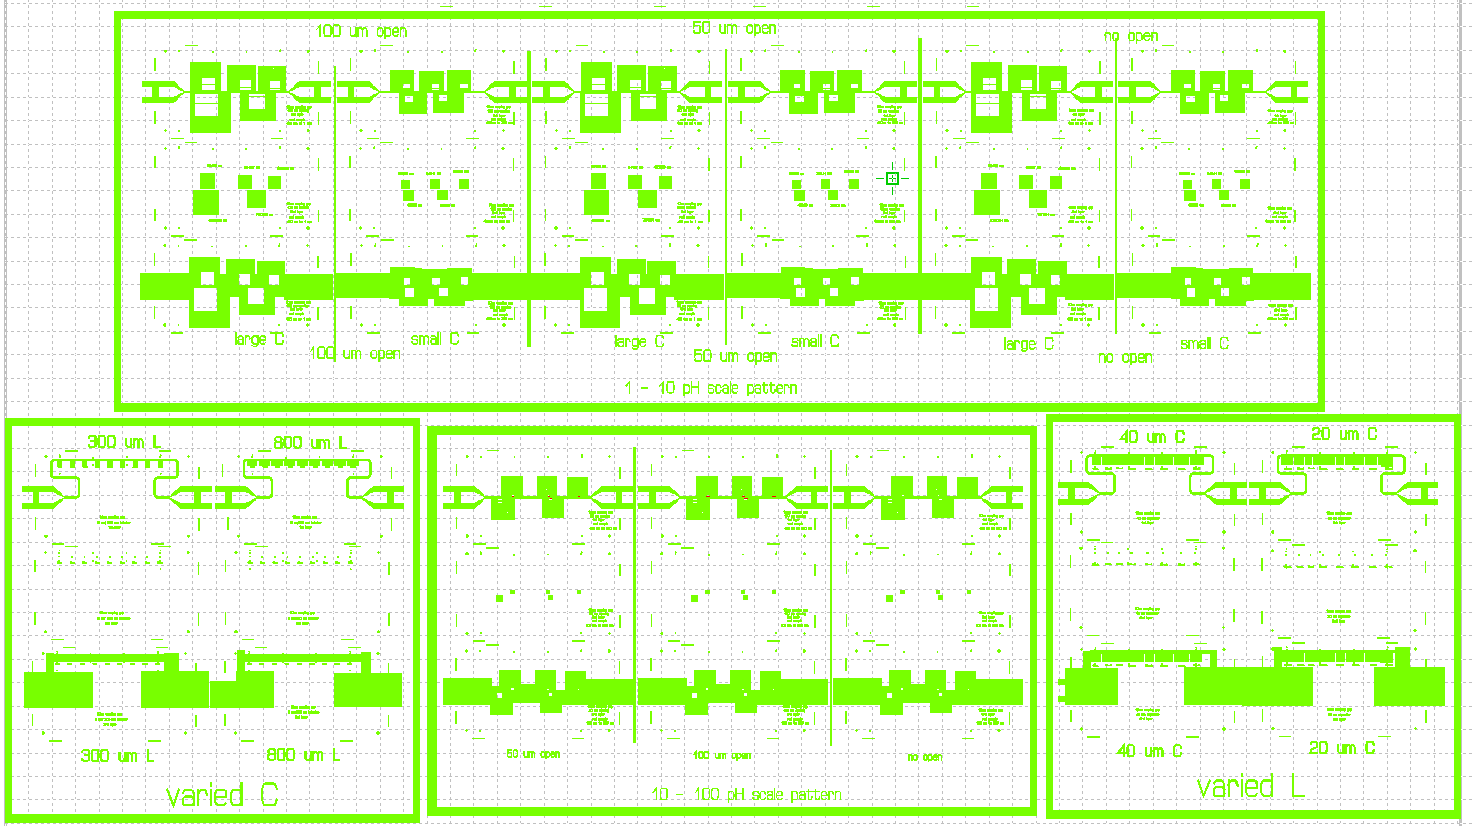
\includegraphics[width=5in]{LC.png}
                \caption{完整的光刻板图案}{}
                \label{fig:LC}
            \end{figure}

            由于没有这类谐振腔的制备经验,对于其频率的估算并没有太多把握,因此我们希望有尽可能多的谐振频率与设计相对应的数据,来辅助下一步对仿真结果的修正与器件制备的改进。由于对电容和电感估值的准确度均有待确认,我们需要至少两组不同的器件设计的组合,一组固定$L$变化$C$的大小,另一组固定$C$变化$L$的大小,这样可以通过拟合确定出每个器件的$L$与$C$的值。因此,一个二维平面波导可以与多个谐振腔耦合,可方便测量。另一方面,考虑到电子束曝光难度与耗时均较大,我们打算先尝试中等数值的电容与电感组合,使电感的尺寸能够通过光刻制备,这样即可在三层电容制备的最后一步同时制作出电感,省去了电子束曝光制备电感的步骤,大大加快样品制备与测试速度。解决三层电容的制备后,再通过电子束曝光制作电感。

            综合上述讨论,我们总共设计了若干种不同的模板几何形状,如图\ref{fig:LC}所示,覆盖了较大范围的电容与电感值,为第一次摸索器件制备工艺以及尝试性测量提供较大的频率变化区间,尽可能保证能够测到谐振腔的共振频率。


            \section{器件制备情况与讨论} % (fold)
            \label{sec:器件制备情况与讨论}
                按照上述计划,我进行了器件制备的工作,目前已完成了完整的器件制备流程。

                
            % section 器件制备 (end)
            



            \section{谐振腔响应信号的拟合} % (fold)
            \label{sec:谐振腔响应信号的拟合}
            	









